\documentclass[11pt,a4paper]{article}

\usepackage[utf8]{inputenc}
\usepackage[T1]{fontenc}
\usepackage[polish]{babel}
\usepackage{lmodern}
\usepackage{microtype}
\usepackage[margin=2.3cm]{geometry}
\usepackage{graphicx}
\usepackage{booktabs}
\usepackage{array}
\usepackage{amsmath}
\usepackage{caption}
\usepackage{xcolor}
\usepackage{hyperref}
\usepackage{listings}
\usepackage{listingsutf8}
\usepackage{enumitem}
\usepackage{float}
\usepackage{tabularx}

\hypersetup{
  colorlinks=true,
  linkcolor=blue!60!black,
  urlcolor=blue!60!black,
  pdftitle={AI Boom Premium},
  pdfauthor={Roksana Kulawiec, Sylwia Malinowska, Mateusz Konopka, Antoni Grabowski}
}

\captionsetup{font=small, labelfont=bf}
\setlist[itemize]{leftmargin=1.4em, itemsep=3pt, topsep=4pt}
\setlist[enumerate]{leftmargin=1.6em, itemsep=3pt, topsep=4pt}
\renewcommand{\arraystretch}{1.15}
\setlength{\tabcolsep}{5pt}

\newcommand{\infobox}[2]{%
  \begin{center}
  \fcolorbox{blue!45!black}{blue!3}{%
    \parbox{0.92\textwidth}{%
      \small\textbf{#1}\par\vspace{3pt}#2%
    }%
  }
  \end{center}
}

\newcommand{\resultbox}[1]{%
  \begin{center}
  \fcolorbox{green!35!black}{green!4}{%
    \parbox{0.92\textwidth}{\small\textbf{Najważniejszy wynik:} #1}%
  }
  \end{center}
}

\newcommand{\cautionbox}[1]{%
  \begin{center}
  \fcolorbox{orange!65!black}{orange!6}{%
    \parbox{0.92\textwidth}{\small\textbf{Uwaga interpretacyjna:} #1}%
  }
  \end{center}
}

\definecolor{codebg}{HTML}{F7F7F7}
\definecolor{codekw}{HTML}{1F4E79}
\definecolor{codestr}{HTML}{8B0000}
\definecolor{codecmt}{HTML}{6B6B6B}

\lstdefinestyle{py}{
  language=Python,
  inputencoding=utf8/latin1,
  extendedchars=true,
  basicstyle=\ttfamily\footnotesize,
  keywordstyle=\color{codekw}\bfseries,
  stringstyle=\color{codestr},
  commentstyle=\color{codecmt}\itshape,
  numbers=left, numberstyle=\tiny\color{gray}, numbersep=6pt,
  backgroundcolor=\color{codebg},
  frame=single, framerule=0pt,
  breaklines=true, breakatwhitespace=true,
  columns=fullflexible, keepspaces=true,
  xleftmargin=12pt, framexleftmargin=10pt,
  showstringspaces=false,
}

\title{\textbf{AI Boom Premium} \\[2pt]
       \large Czy spółki silnie powiązane z infrastrukturą AI osiągnęły wyższe
       średnie zwroty i lepszy profil ryzyko--zwrot po rozpoczęciu boomu
       generatywnej AI? \\[6pt]
       \normalsize \emph{Projekt zaliczeniowy IAD --- Metody Badań w Finansach,
       ćwiczenia 3}}
\author{%
  Roksana Kulawiec (454474) \\
  Sylwia Malinowska (487648) \\
  Mateusz Konopka (487528) \\
  Antoni Grabowski (452622)%
}
\date{\today}

\begin{document}
\maketitle

\infobox{Repozytorium kodu i danych}{
\href{https://github.com/Smalou/metody_badania_w_finansach}{\texttt{github.com/Smalou/metody\_badania\_w\_finansach}} \\
Wszystkie skrypty Pythona, cache danych (\texttt{parquet}/\texttt{csv}),
wygenerowane wykresy i źródło niniejszego raportu LaTeX są dostępne
w powyższym repozytorium.}

\infobox{Streszczenie dla czytelnika}{
Raport sprawdza, czy po premierze ChatGPT spółki infrastruktury AI osiągały
wyższe zwroty ponad benchmark SPY i lepszy profil ryzyko--zwrot niż grupy
kontrolne. Wszystkie trzy zadania wskazują na przewagę segmentu
\textbf{AI infrastructure}, ale wyniki są historyczne, ex post i nie stanowią
prognozy przyszłych stóp zwrotu.}

\tableofcontents
\clearpage

% =====================================================================
\section*{Wprowadzenie i hipoteza projektowa}

W projekcie przyjęto premierę ChatGPT (30 listopada 2022) jako symboliczny punkt
startu masowej fazy boomu generatywnej AI. W kolejnych kwartałach temat AI stał
się jednym z głównych motywów inwestycyjnych na rynku amerykańskim, szczególnie
w segmencie półprzewodników, infrastruktury obliczeniowej i usług chmurowych.
Niniejszy projekt sprawdza empirycznie, czy po tej dacie wystąpiły mierzalne
różnice w średnich zwrotach oraz profilu ryzyko--zwrot między spółkami o różnym
stopniu ekspozycji na sztuczną inteligencję. Analiza ma charakter statystyczny
i porównawczy; nie jest dowodem przyczynowym w ścisłym sensie ekonometrycznym.

\paragraph{Główna teza.} \emph{Spółki silnie powiązane z infrastrukturą AI
(producenci półprzewodników i sprzętu) osiągnęły po 30.11.2022 istotnie wyższe
średnie zwroty względem benchmarku rynkowego (SPY) oraz lepszy profil
ryzyko--zwrot niż grupy kontrolne (Defensive, Broad Tech, AI Platforms).}

\paragraph{Trzy zadania spójne tematycznie.}
\begin{itemize}
  \item \textbf{Zadanie 1} --- porównanie średnich miesięcznych \emph{abnormal
        returns} (AR względem SPY) portfela AI infrastructure i portfela
        Defensive control \emph{po} rozpoczęciu boomu (próby niezależne).
  \item \textbf{Zadanie 2} --- porównanie średnich metryk efektywności
        ryzyko--zwrot (\emph{Sharpe Ratio} jako zmienna główna, \emph{CAPM alpha}
        jako uzupełnienie) między czterema grupami spółek.
  \item \textbf{Zadanie 3} --- A/B testing na próbach zależnych: średnie dzienne
        AR tej samej spółki w oknie przed (wariant A) i po (wariant B) 30.11.2022,
        z analizą wrażliwości na długość okna i \emph{placebo test}.
\end{itemize}

\paragraph{Dane.} Źródło: Yahoo Finance przez bibliotekę \texttt{yfinance}.
41 spółek notowanych na NYSE/NASDAQ podzielonych na cztery grupy (definicje w
\texttt{data\_cache/metadata\_tickers.csv}) plus benchmark \texttt{SPY} i stopa
wolna od ryzyka \texttt{\textasciicircum IRX} (13-tygodniowy T-bill).
Okres: 04.01.2021--14.05.2026 (1347 dni sesyjnych). Ceny skorygowane
(\texttt{auto\_adjust=True}), brak braków danych.

\paragraph{Grupy spółek (11+10+10+10 = 41).}
\begin{itemize}
  \item \textbf{AI infrastructure / półprzewodniki (11)}: NVDA, AMD, AVGO, TSM,
        ASML, AMAT, LRCX, KLAC, MU, MRVL, SMCI.
  \item \textbf{AI platforms / cloud / software (10)}: MSFT, GOOGL, AMZN, META,
        ORCL, CRM, NOW, ADBE, IBM, SNOW.
  \item \textbf{Broad technology control (10)}: AAPL, CSCO, INTC, TXN, QCOM,
        INTU, ACN, PANW, CDNS, ADSK.
  \item \textbf{Defensive control (10)}: KO, PEP, PG, WMT, JNJ, MRK, MCD, COST,
        CL, GIS.
\end{itemize}

\paragraph{Kontekst graficzny --- skumulowane abnormal returns per grupa.}
Poniższy wykres przedstawia skumulowany dzienny abnormal return portfela
równoważonego (EW) każdej grupy względem SPY. Pionowa linia oznacza moment
zdarzenia 30.11.2022.

\begin{center}
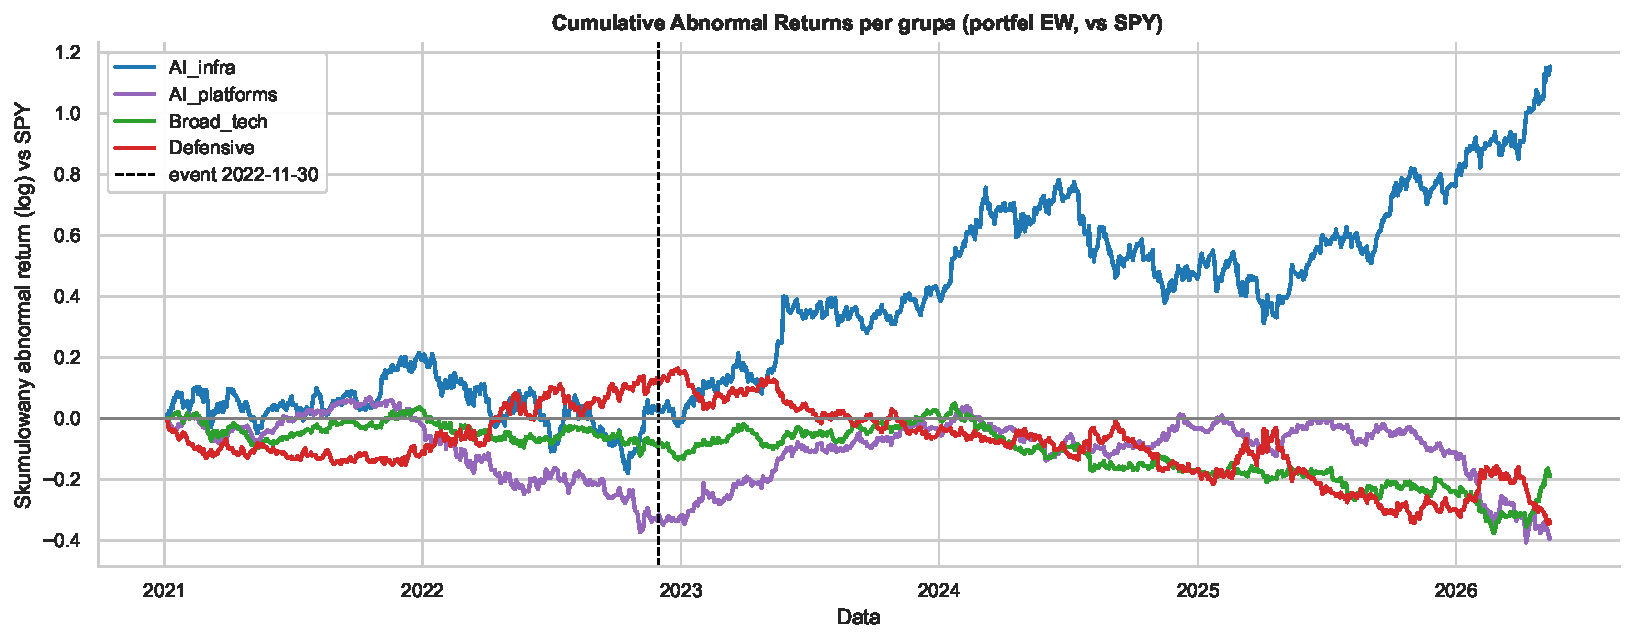
\includegraphics[width=\textwidth]{../figures/extra_cumulative_AR.pdf}
\end{center}

Widoczne jest wyraźne rozejście trajektorii AI infrastructure od pozostałych grup
po listopadzie 2022. Wykres pełni jednak wyłącznie funkcję diagnostyczną i
opisową; formalne wnioski oparto na testach statystycznych, wielkościach efektu
i analizach odporności przedstawionych w trzech zadaniach poniżej.

\cautionbox{Wykres skumulowanych AR pomaga zrozumieć kontekst, ale nie zastępuje
testów statystycznych. Formalne decyzje w raporcie opierają się na testach,
przedziałach ufności i wielkościach efektu.}

\clearpage
% =====================================================================
\section{Zadanie 1 --- AI infrastructure vs Defensive: miesięczne abnormal returns}

\subsection{Opis zmiennych}
Dla każdej grupy zbudowano portfel równoważony (EW). Dzienna stopa zwrotu
portfela:
\[
 r_t^{\text{port}} = \frac{1}{N} \sum_{i=1}^N r_{i,t},
\]
gdzie $r_{i,t}$ to dzienna log-stopa zwrotu spółki $i$. Następnie:
\begin{itemize}
  \item agregacja miesięczna: $r^{\text{port}}_m = \sum_{t \in m} r^{\text{port}}_t$
        (suma log-zwrotów, ekwiwalentnie miesięczny log-zwrot);
  \item \emph{abnormal return}: $AR^{\text{port}}_m = r^{\text{port}}_m - r^{\text{SPY}}_m$;
  \item filtracja czasowa: tylko obserwacje \emph{po} 30.11.2022.
\end{itemize}

Porównywane zmienne (próby niezależne, $n_1 = n_2 = 42$ miesiące):
\begin{itemize}
  \item $X$: miesięczne AR portfela \textbf{AI infrastructure} (11 spółek),
  \item $Y$: miesięczne AR portfela \textbf{Defensive control} (10 spółek).
\end{itemize}
Ostatni miesiąc w próbie (maj 2026) jest miesiącem częściowym ze względu na datę
pobrania danych. W głównym wyniku zachowano go dla zgodności z cache danych;
w praktycznej analizie inwestycyjnej warto dodatkowo sprawdzić wariant z jego
wykluczeniem.

\subsection{Hipotezy badawcze}
\begin{itemize}
  \item $H_0$: średnie miesięczne AR obu portfeli są równe,
        $\mu_{AR,\text{AI}} = \mu_{AR,\text{Def}}$.
  \item $H_1$: średnie różnią się, $\mu_{AR,\text{AI}} \neq \mu_{AR,\text{Def}}$.
\end{itemize}

\subsection{Procedura statystyczna}
\begin{enumerate}
  \item Sprawdzenie założeń: Shapiro-Wilk (normalność) + Levene (homogeniczność
        wariancji).
  \item \textbf{Test główny}: \emph{Welch t-test} dla dwóch prób niezależnych
        (bez założenia równych wariancji).
  \item \textbf{Analiza odporności}: bootstrap (B~=~10\,000, ziarno 42)
        95\% przedziału ufności różnicy średnich.
  \item Wielkość efektu: \emph{Hedges' g} (poprawiona Cohen's $d$ dla małych
        prób).
  \item \textbf{Test pomocniczy}: Mann-Whitney U --- różnica w położeniu rozkładów
        (\emph{nie} test średnich, dla kompletności).
\end{enumerate}

\subsection{Kod źródłowy (fragment)}
\lstinputlisting[style=py, firstline=28, lastline=70]{../src_ascii/task1_two_portfolios.py}

\subsection{Wyniki}
\paragraph{Statystyki opisowe.}
\begin{center}\small
\begin{tabular}{lrrr}
\toprule
Portfel & $n$ & średnia $AR_m$ & odch. std. \\
\midrule
AI infrastructure & 42 & $\phantom{-}0{,}02638$ & $0{,}07774$ \\
Defensive control & 42 & $-0{,}01089$ & $0{,}04133$ \\
\bottomrule
\end{tabular}
\end{center}

\paragraph{Założenia.}
\begin{itemize}
  \item Shapiro-Wilk AI infra: $W = 0{,}956;\ p = 0{,}1053$ (rozkład zbliżony do
        normalnego);
  \item Shapiro-Wilk Defensive: $W = 0{,}987;\ p = 0{,}9141$ (rozkład zbliżony do
        normalnego);
  \item Levene (median): $\text{stat} = 13{,}23;\ p = 0{,}0005$ (wariancje
        istotnie różne $\rightarrow$ uzasadnia \emph{Welch}, a nie klasyczny
        $t$-Student).
\end{itemize}

\paragraph{Test główny --- Welch t-test, bootstrap i Mann-Whitney.}
\begin{center}\small
\begin{tabular}{lrl}
\toprule
Test & wartość & uwaga \\
\midrule
Welch $t$ ($\mathrm{df} \approx 62{,}5$) & $2{,}744$ & \\
$p$-value & $0{,}00792$ & odrzucenie $H_0$ \\
Różnica średnich ($\bar X - \bar Y$) & $+0{,}03728$ & na korzyść AI infra \\
95\% CI (Welch) & $[+0{,}01012;\ +0{,}06443]$ & nie zawiera 0 \\
Hedges' $g$ & $+0{,}593$ & umiarkowany efekt \\
\midrule
95\% CI bootstrap (B~=~10\,000) & $[+0{,}01199;\ +0{,}06365]$ & spójne z Welch \\
\midrule
Mann-Whitney $U$ (\emph{pomocniczy}) & $1122{,}0$ & różnica w położeniu rozkładów \\
$p$-value (M-W) & $0{,}0321$ & spójne z $H_1$ \\
\bottomrule
\end{tabular}
\end{center}

\resultbox{Portfel AI infrastructure miał średnio o $+3{,}73$ p.p. miesięcznie
wyższy abnormal return niż portfel Defensive, a 95\% przedziały ufności nie
obejmują zera.}

\paragraph{Wykres rozkładów.}
\begin{center}
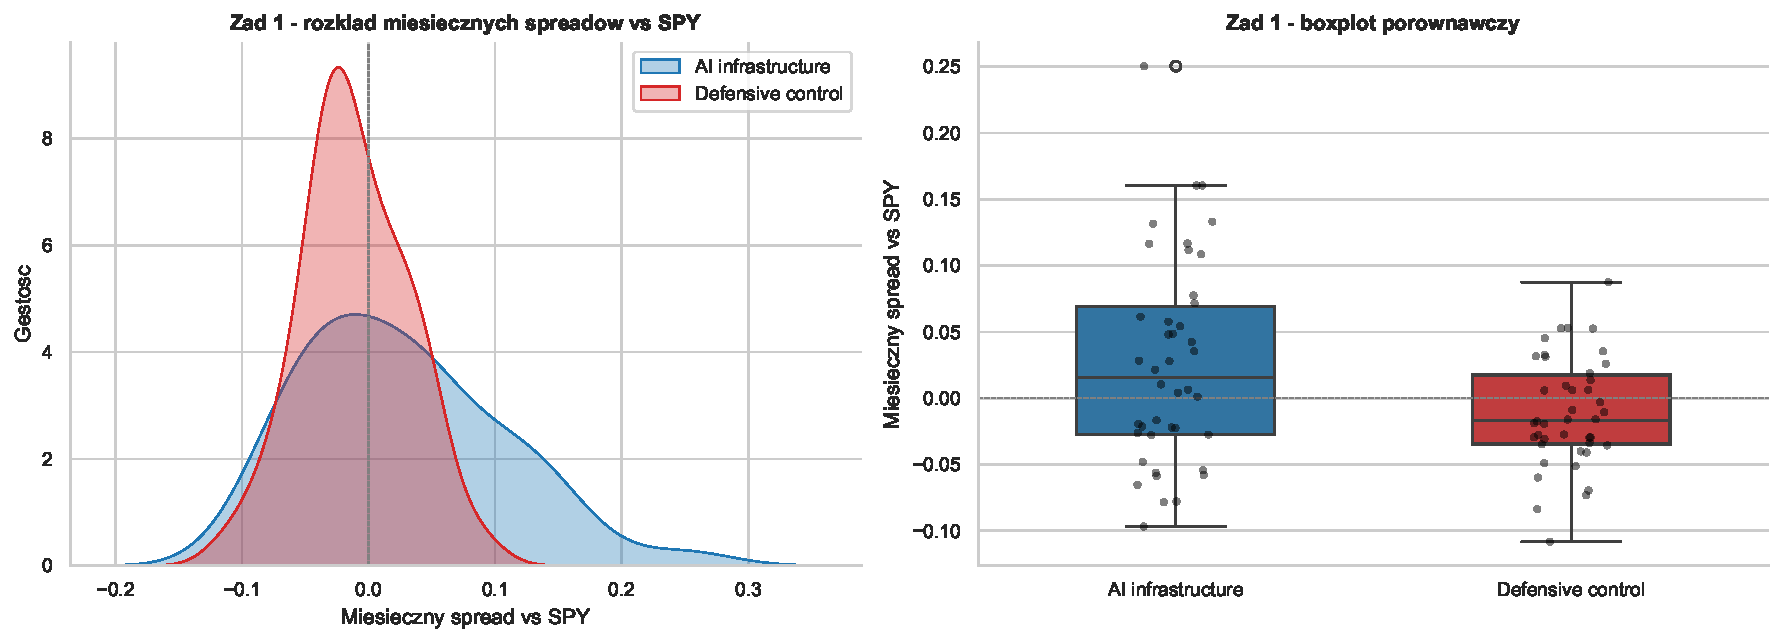
\includegraphics[width=\textwidth]{../figures/task1_distributions.pdf}
\end{center}

\subsection{Interpretacja}
\begin{itemize}
  \item \textbf{Zmienna}: miesięczny abnormal return portfela EW vs SPY,
        $n = 42$ miesięcy (12.2022--05.2026).
  \item \textbf{Test zastosowany}: Welch t-test (główny) + bootstrap (odporność)
        + Mann-Whitney U (pomocniczy).
  \item \textbf{Wynik}: $p = 0{,}0079$; $\bar X - \bar Y = +3{,}73$ p.p.
        miesięcznie; 95\% CI Welch $[+1{,}01;\ +6{,}44]$ p.p.; Hedges' $g = 0{,}59$.
        Bootstrap CI praktycznie pokrywa się z Welch.
  \item \textbf{Decyzja statystyczna}: odrzucamy $H_0$ przy $\alpha = 0{,}05$.
  \item \textbf{Interpretacja ekonomiczna}: w okresie 42 miesięcy po premierze
        ChatGPT portfel AI infrastructure dostarczył średnio ok. 3{,}7 p.p.
        \emph{na miesiąc} wyższego abnormal returnu względem SPY niż portfel
        defensywny. Wynik jest spójny z hipotezą \emph{AI Boom Premium},
        choć wyższa zmienność portfela AI ($\sigma = 7{,}8\%$) wskazuje, że
        premia ta wiąże się z istotnie większym ryzykiem (do oceny w Zadaniu 2).
\end{itemize}

\cautionbox{Wynik z Zadania 1 pokazuje istotną różnicę średnich AR, ale portfel
AI infrastructure miał też wyraźnie wyższą zmienność. Dlatego sama premia zwrotu
nie wystarcza do decyzji inwestycyjnej bez oceny ryzyka.}

\clearpage
% =====================================================================
\section{Zadanie 2 --- Metryki efektywności w czterech grupach spółek}

\subsection{Opis zmiennych}
Dla każdej z 41 spółek obliczono komplet 7 metryk na bazie dziennych log-zwrotów
za cały okres 04.01.2021--14.05.2026:
\begin{itemize}
  \item \emph{Annualized return} $= \bar r_t \cdot 252$,
  \item \emph{Annualized volatility} $= s(r_t) \cdot \sqrt{252}$,
  \item \emph{Sharpe Ratio} $= \overline{(r_t - r_f)} / s(r_t - r_f) \cdot \sqrt{252}$,
  \item \emph{Sortino Ratio} (downside deviation względem MAR~=~0),
  \item \emph{Maximum drawdown} liczony na wealth-curve $\exp(\sum r_t)$,
  \item \emph{CAPM beta} z regresji nadwyżkowych zwrotów na SPY,
  \item \emph{CAPM alpha} (annualized).
\end{itemize}

\paragraph{Główna zmienna testowana}: \textbf{Sharpe Ratio} (najszerzej akceptowana
miara ryzyko--zwrot w finansach). Dla kompletności --- równolegle ten sam test
przeprowadzono dla \textbf{CAPM alpha}, bezpośrednio mierzącego ,,nadwyżkę po
kontroli ryzyka systematycznego'' i najbliższego pojęciu \emph{AI Premium}.

\paragraph{Statystyki opisowe (średnie metryk per grupa).}
\begin{center}\small
\begin{tabular}{lrrrrrr}
\toprule
Grupa & Ann.~ret & Ann.~vol & Sharpe & Sortino & Max DD & alpha \\
\midrule
AI infrastructure & $0{,}362$ & $0{,}501$ & $\mathbf{0{,}674}$ & $0{,}684$ & $-0{,}584$ & $\mathbf{+0{,}119}$ \\
AI platforms      & $0{,}072$ & $0{,}374$ & $0{,}154$ & $0{,}159$ & $-0{,}567$ & $-0{,}107$ \\
Broad tech        & $0{,}111$ & $0{,}349$ & $0{,}228$ & $0{,}228$ & $-0{,}452$ & $-0{,}064$ \\
Defensive         & $0{,}082$ & $0{,}192$ & $0{,}250$ & $0{,}244$ & $-0{,}297$ & $+0{,}011$ \\
\bottomrule
\end{tabular}
\end{center}

\subsection{Hipotezy badawcze}
\begin{itemize}
  \item $H_0$: średnie Sharpe Ratio (alpha) są równe we wszystkich czterech
        grupach.
  \item $H_1$: co najmniej jedna grupa ma średnią różną od pozostałych.
\end{itemize}

\subsection{Procedura statystyczna --- drzewo decyzyjne}
\begin{enumerate}
  \item Shapiro-Wilk per grupa $\rightarrow$ czy rozkłady normalne?
  \item Levene (median) $\rightarrow$ czy wariancje jednorodne?
  \item Decyzja:
        \begin{itemize}
          \item normalne + jednorodne $\rightarrow$ \textbf{ANOVA} + Tukey HSD,
          \item normalne + nierówne wariancje $\rightarrow$ \textbf{Welch ANOVA}
                + Games-Howell,
          \item nienormalne $\rightarrow$ \textbf{Kruskal-Wallis} + Dunn
                (Bonferroni).
        \end{itemize}
  \item Wielkość efektu: $\eta^2$ i $\omega^2$ (mniej obciążone dla małych prób).
\end{enumerate}

\subsection{Kod źródłowy (fragment)}
\lstinputlisting[style=py, firstline=23, lastline=86]{../src_ascii/task2_four_groups.py}

\subsection{Wyniki --- zmienna główna: Sharpe Ratio}

\paragraph{Założenia.}
Shapiro-Wilk: wszystkie cztery grupy spełniają normalność ($p > 0{,}05$).
Levene: $\text{stat} = 1{,}25;\ p = 0{,}299$ --- wariancje jednorodne. Decyzja:
\textbf{ANOVA + Tukey HSD}.

\paragraph{ANOVA jednoczynnikowa.}
$F(3,\ 37) = 4{,}956;\quad p = 0{,}00543;\quad \eta^2 = 0{,}287;\ \omega^2 = 0{,}225$.
Odrzucamy $H_0$. Wartość $\omega^2 \approx 0{,}22$ wskazuje na duży efekt
(konwencja Cohena: $\omega^2 \geq 0{,}14$ duży).

\paragraph{Tukey HSD (FWER $= 0{,}05$).} Różnica oznacza średnią grupy 1 minus średnią grupy 2.
\begin{center}\small
\begin{tabular}{llrrrl}
\toprule
Grupa 1 & Grupa 2 & różnica (1--2) & $p_\text{adj}$ & 95\% CI & istotne \\
\midrule
AI infra     & AI platforms & $+0{,}519$ & $0{,}0076$ & $[+0{,}113;\ +0{,}925]$ & \textbf{tak} \\
AI infra     & Broad tech   & $+0{,}445$ & $0{,}0269$ & $[+0{,}039;\ +0{,}851]$ & \textbf{tak} \\
AI infra     & Defensive    & $+0{,}424$ & $0{,}0380$ & $[+0{,}018;\ +0{,}829]$ & \textbf{tak} \\
AI platforms & Broad tech   & $-0{,}074$ & $0{,}9633$ & $[-0{,}489;\ +0{,}341]$ & nie \\
AI platforms & Defensive    & $-0{,}096$ & $0{,}9253$ & $[-0{,}511;\ +0{,}320]$ & nie \\
Broad tech   & Defensive    & $-0{,}022$ & $0{,}9990$ & $[-0{,}437;\ +0{,}394]$ & nie \\
\bottomrule
\end{tabular}
\end{center}

\resultbox{AI infrastructure ma istotnie wyższy średni Sharpe Ratio niż każda
z trzech pozostałych grup. Między AI platforms, Broad tech i Defensive nie
widać istotnych różnic w parach.}

\paragraph{Wykres --- Sharpe per grupa.}
\begin{center}
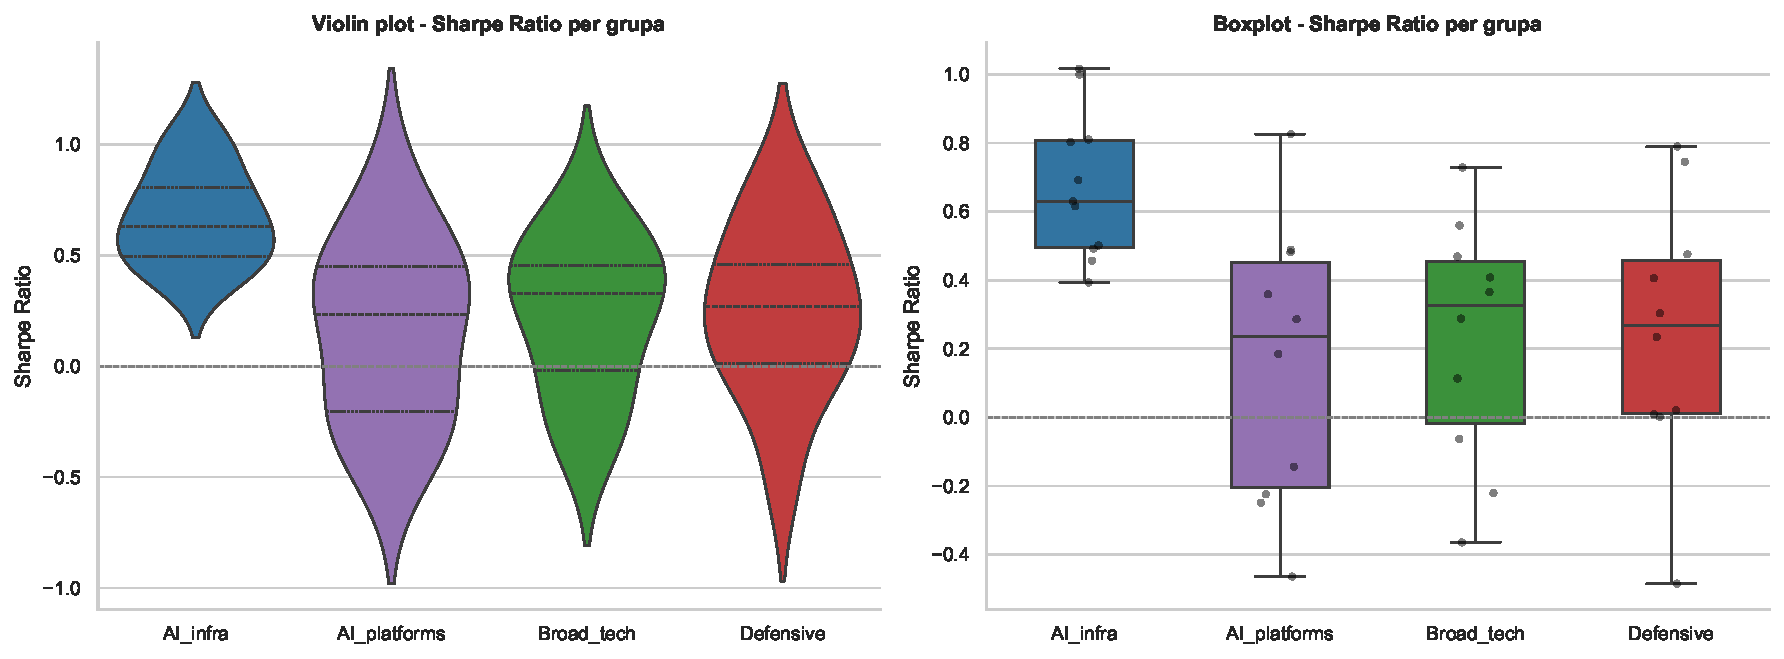
\includegraphics[width=\textwidth]{../figures/task2_sharpe_per_group.pdf}
\end{center}

\subsection{Wyniki --- zmienna uzupełniająca: CAPM alpha}

\paragraph{Założenia.}
Wszystkie grupy spełniają normalność (Shapiro $p > 0{,}05$); Levene
$\text{stat} = 2{,}57;\ p = 0{,}066$ --- nieznacznie powyżej $\alpha$,
wariancje uznajemy za jednorodne. Decyzja: \textbf{ANOVA + Tukey HSD}.

\paragraph{ANOVA jednoczynnikowa.}
$F(3,\ 37) = 7{,}621;\quad p = 4{,}3 \cdot 10^{-4};\quad \eta^2 = 0{,}382;\
\omega^2 = 0{,}326$. Odrzucamy $H_0$ z silnym efektem ($\omega^2 \approx 0{,}33$).

\paragraph{Tukey HSD (FWER $= 0{,}05$).} Różnica oznacza średnią grupy 1 minus średnią grupy 2.
\begin{center}\small
\begin{tabular}{llrrrl}
\toprule
Grupa 1 & Grupa 2 & różnica $\alpha$ (1--2) & $p_\text{adj}$ & 95\% CI & istotne \\
\midrule
AI infra     & AI platforms & $+0{,}226$ & $0{,}0004$ & $[+0{,}089;\ +0{,}363]$ & \textbf{tak} \\
AI infra     & Broad tech   & $+0{,}183$ & $0{,}0049$ & $[+0{,}046;\ +0{,}320]$ & \textbf{tak} \\
AI infra     & Defensive    & $+0{,}108$ & $0{,}1665$ & $[-0{,}029;\ +0{,}245]$ & nie \\
AI platforms & Broad tech   & $-0{,}043$ & $0{,}8450$ & $[-0{,}183;\ +0{,}098]$ & nie \\
AI platforms & Defensive    & $-0{,}118$ & $0{,}1247$ & $[-0{,}259;\ +0{,}022]$ & nie \\
Broad tech   & Defensive    & $-0{,}076$ & $0{,}4791$ & $[-0{,}216;\ +0{,}065]$ & nie \\
\bottomrule
\end{tabular}
\end{center}

\resultbox{Dla CAPM alpha przewaga AI infrastructure jest istotna względem
AI platforms i Broad tech, ale nie względem Defensive. To sugeruje, że sama
premia AI nie jest równomiernie rozłożona między wszystkie spółki technologiczne.}

\paragraph{Wykres --- CAPM alpha per grupa.}
\begin{center}
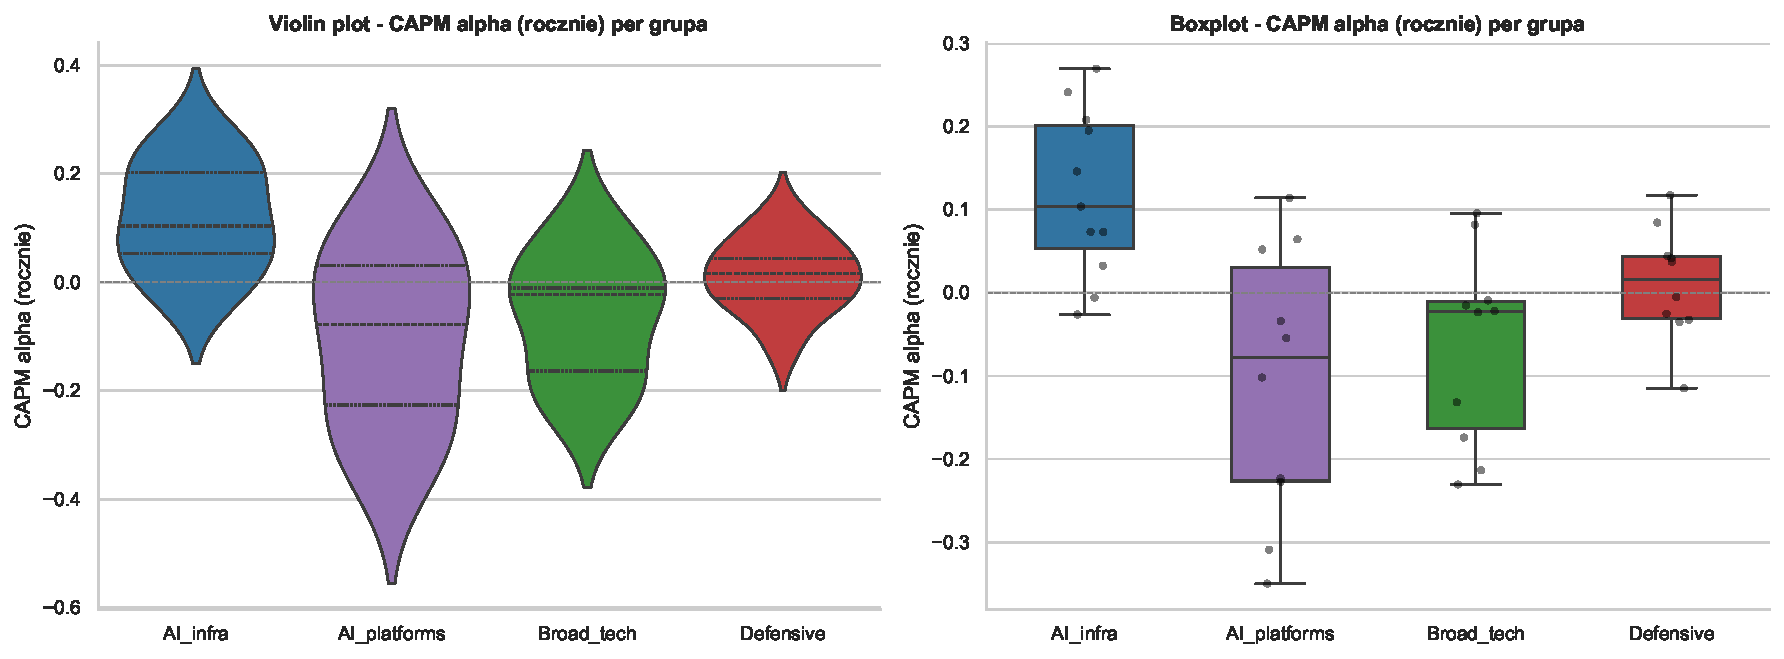
\includegraphics[width=\textwidth]{../figures/task2_alpha_per_group.pdf}
\end{center}

\paragraph{Forest plot --- różnice metryk vs grupa Defensive.}
\begin{center}
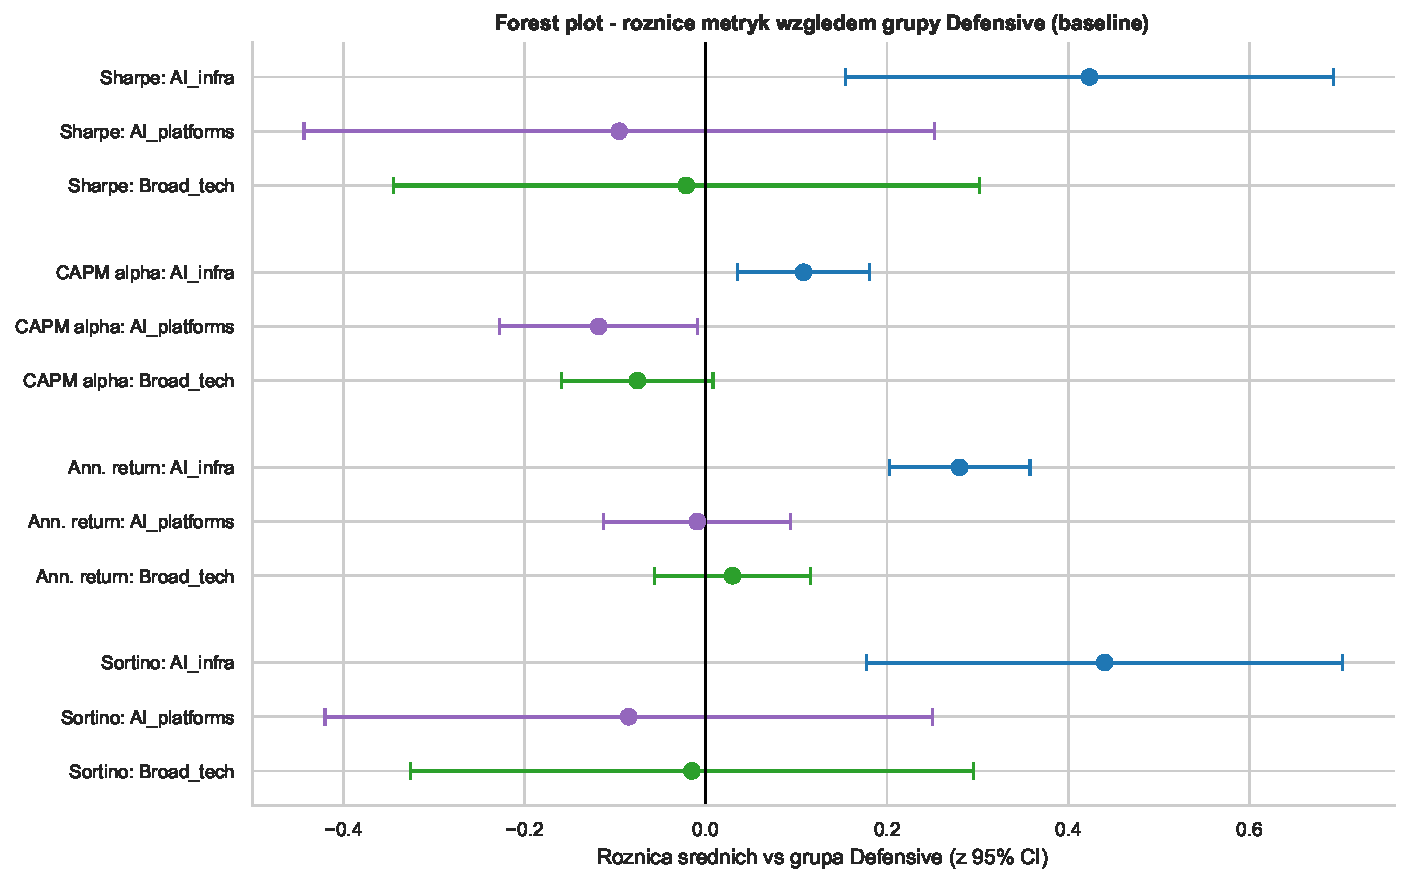
\includegraphics[width=0.85\textwidth]{../figures/extra_forest_diff.pdf}
\end{center}

\subsection{Interpretacja}
\begin{itemize}
  \item \textbf{Zmienna}: Sharpe Ratio (główna) oraz CAPM alpha (uzupełniająca)
        liczone per spółka na dziennych log-zwrotach 2021--2026; $n = 41$
        spółek w 4 grupach.
  \item \textbf{Test zastosowany}: ANOVA + Tukey HSD (oba przypadki: założenia
        spełnione).
  \item \textbf{Wynik (Sharpe)}: $F(3,37) = 4{,}96;\ p = 0{,}005;\ \omega^2 = 0{,}23$.
        Tukey lokalizuje różnice: AI infrastructure ma istotnie wyższy średni
        Sharpe Ratio niż każda z pozostałych grup; pozostałe trzy grupy nie
        różnią się między sobą.
  \item \textbf{Wynik (alpha)}: $F(3,37) = 7{,}62;\ p = 4{,}3 \cdot 10^{-4};\
        \omega^2 = 0{,}33$. AI infrastructure ma istotnie wyższą $\alpha$ niż
        AI platforms i Broad tech; różnica względem Defensive jest dodatnia, ale
        nie osiąga istotności statystycznej ($p = 0{,}17$). Defensive ma
        $\alpha \approx 0$, przy wyraźnie niższym poziomie ryzyka.
  \item \textbf{Decyzja statystyczna}: odrzucamy $H_0$ w obu testach.
  \item \textbf{Interpretacja ekonomiczna}: wyniki sugerują, że premia AI ma
        wyraźny charakter \emph{sektorowy} (półprzewodniki i sprzęt) ---
        platformy chmurowe (MSFT, GOOGL, AMZN itd.) nie wyróżniły się istotnie
        ani Sharpe Ratio, ani $\alpha$ względem reszty rynku. Jedna z możliwych
        interpretacji jest taka, że hyperscalerzy ponoszą wysokie nakłady
        inwestycyjne na infrastrukturę AI, natomiast dostawcy półprzewodników
        i sprzętu są jej bezpośrednimi beneficjentami przychodowymi.
\end{itemize}

\paragraph{Ograniczenie próby.}
Liczebności grup są niewielkie i nierówne (11 spółek w AI infrastructure oraz po
10 spółek w pozostałych grupach). Jest to próba dobrana \emph{celowo}
(reprezentatywne spółki z ekspozycją na dany typ ryzyka/tematu inwestycyjnego),
a nie losowo z populacji. Wnioski statystyczne dotyczą analizowanej próby i
okresu 2021--2026 --- nie należy ich uogólniać na ,,cały rynek''. Dodatkowo
grupy Broad tech i Defensive są sektorowo niejednorodne wewnętrznie, co zwiększa
wariancję wewnątrzgrupową i tym samym zmniejsza moc testu.

\clearpage
% =====================================================================
\section{Zadanie 3 --- A/B testing na próbach zależnych wokół 30.11.2022}

\subsection{Opis zmiennych i schemat A/B}
Zdarzenie: \textbf{publiczna premiera ChatGPT, 30.11.2022} --- przyjęta jako data
rozpoczęcia masowej fazy boomu generatywnej AI. Próba: 21 spółek z połączonej
grupy ,,AI'' = AI infrastructure $\cup$ AI platforms (11 + 10 = 21 spółek).

Dla każdej spółki $i$ liczymy dwie wartości:
\begin{itemize}
  \item \textbf{Wariant A}: $\bar{AR}_i^{(A)}$ --- średni dzienny abnormal return
        (vs SPY) w oknie $K$ sesji \emph{przed} 30.11.2022,
  \item \textbf{Wariant B}: $\bar{AR}_i^{(B)}$ --- średni dzienny abnormal return
        w oknie $K$ sesji \emph{po} 30.11.2022.
\end{itemize}
Jednostką pary jest \emph{ta sama spółka}. Próby są więc zależne (paired).
Statystyka testowa: $d_i = \bar{AR}_i^{(B)} - \bar{AR}_i^{(A)}$.

\subsection{Hipotezy badawcze}
\begin{itemize}
  \item $H_0$: $\mu_d = 0$ --- średnia różnica AR między wariantem B i A wynosi
        zero.
  \item $H_1$: $\mu_d \neq 0$.
\end{itemize}

\subsection{Procedura statystyczna}
\begin{enumerate}
  \item Test normalności różnic $d_i$ (Shapiro-Wilk).
  \item \textbf{Test główny}: paired $t$-test (jeśli różnice normalne).
  \item \textbf{Test odporności}: Wilcoxon signed-rank (zawsze raportowany).
        W przypadku odrzucenia normalności Wilcoxon staje się testem głównym.
  \item Wielkość efektu: Cohen's $d_z = \bar d / s_d$; 95\% przedział ufności
        dla $\bar d$ (rozkład $t$ z $n - 1$ stopniami swobody).
  \item \textbf{Analiza wrażliwości} na długość okna: $K \in \{30, 60, 120, 250\}$
        sesji. Okno bazowe: $K = 120$ (~6 miesięcy ekspozycji \emph{ex post}).
  \item \textbf{Placebo test}: cała procedura powtórzona dla daty 30.11.2021
        (rok przed boomem AI). Jeżeli wynik dla eventu nie pojawia się
        ,,przypadkowo'', placebo nie powinien dawać analogicznie istotnego
        efektu \emph{w tym samym kierunku}.
\end{enumerate}

\subsection{Kod źródłowy (fragment)}
\lstinputlisting[style=py, firstline=29, lastline=82]{../src_ascii/task3_paired_event.py}

\subsection{Wyniki}

\paragraph{Główny test --- okno bazowe $K = 120$ sesji.}
Shapiro-Wilk: $W = 0{,}897;\ p = 0{,}0227$ --- różnice odbiegają od rozkładu
normalnego, więc testem głównym jest Wilcoxon, a paired $t$-test raportujemy
jako wspierający.
\[
\bar d = +0{,}00243;\quad
\text{95\% CI: } [+0{,}00123;\ +0{,}00363];\quad
 d_z = +0{,}92\ \text{(duży efekt)};
\]
\[
\text{Wilcoxon } p = 8{,}4 \cdot 10^{-5};\quad
\text{paired } t(20) = 4{,}11;\ p = 4{,}2 \cdot 10^{-4}.
\]
Oba testy zgodnie odrzucają $H_0$.

\resultbox{W oknie bazowym 120 sesji średnia różnica po--przed jest dodatnia
i istotna statystycznie. Efekt pojawia się mocno dopiero w dłuższych oknach,
co jest spójne z narastającą wyceną tematu AI po premierze ChatGPT.}

\paragraph{Pełna analiza wrażliwości + placebo.}
\begin{center}\small
\begin{tabular}{lrrrrrl}
\toprule
Wariant & $K$ & $\bar d$ & 95\% CI & $d_z$ & $p$ (główny) & test \\
\midrule
\multicolumn{7}{l}{\textbf{Event: 30.11.2022 (premiera ChatGPT)}} \\
event & 30  & $-0{,}00177$ & $[-0{,}00502;\ +0{,}00149]$ & $-0{,}25$ & $0{,}2707$ & paired $t$ \\
event & 60  & $+0{,}00147$ & $[-0{,}00024;\ +0{,}00317]$ & $+0{,}39$ & $0{,}0760$ & Wilcoxon \\
event & \textbf{120} & $\mathbf{+0{,}00243}$ & $\mathbf{[+0{,}00123;\ +0{,}00363]}$ & $\mathbf{+0{,}92}$ & $\mathbf{8{,}4 \cdot 10^{-5}}$ & Wilcoxon \\
event & 250 & $+0{,}00231$ & $[+0{,}00143;\ +0{,}00319]$ & $+1{,}20$ & $< 10^{-4}$ & paired $t$ \\
\midrule
\multicolumn{7}{l}{\textbf{Placebo: 30.11.2021 (rok przed boomem AI)}} \\
placebo & 30  & $-0{,}00385$ & $[-0{,}00672;\ -0{,}00098]$ & $-0{,}61$ & $0{,}0110$ & paired $t$ \\
placebo & 60  & $-0{,}00290$ & $[-0{,}00447;\ -0{,}00134]$ & $-0{,}84$ & $0{,}0010$ & paired $t$ \\
placebo & 120 & $-0{,}00260$ & $[-0{,}00412;\ -0{,}00108]$ & $-0{,}78$ & $0{,}0020$ & paired $t$ \\
placebo & 250 & $-0{,}00156$ & $[-0{,}00248;\ -0{,}00064]$ & $-0{,}77$ & $0{,}0021$ & paired $t$ \\
\bottomrule
\end{tabular}
\end{center}

\paragraph{Wykres --- histogram różnic + sensitivity z placebo.}
\begin{center}
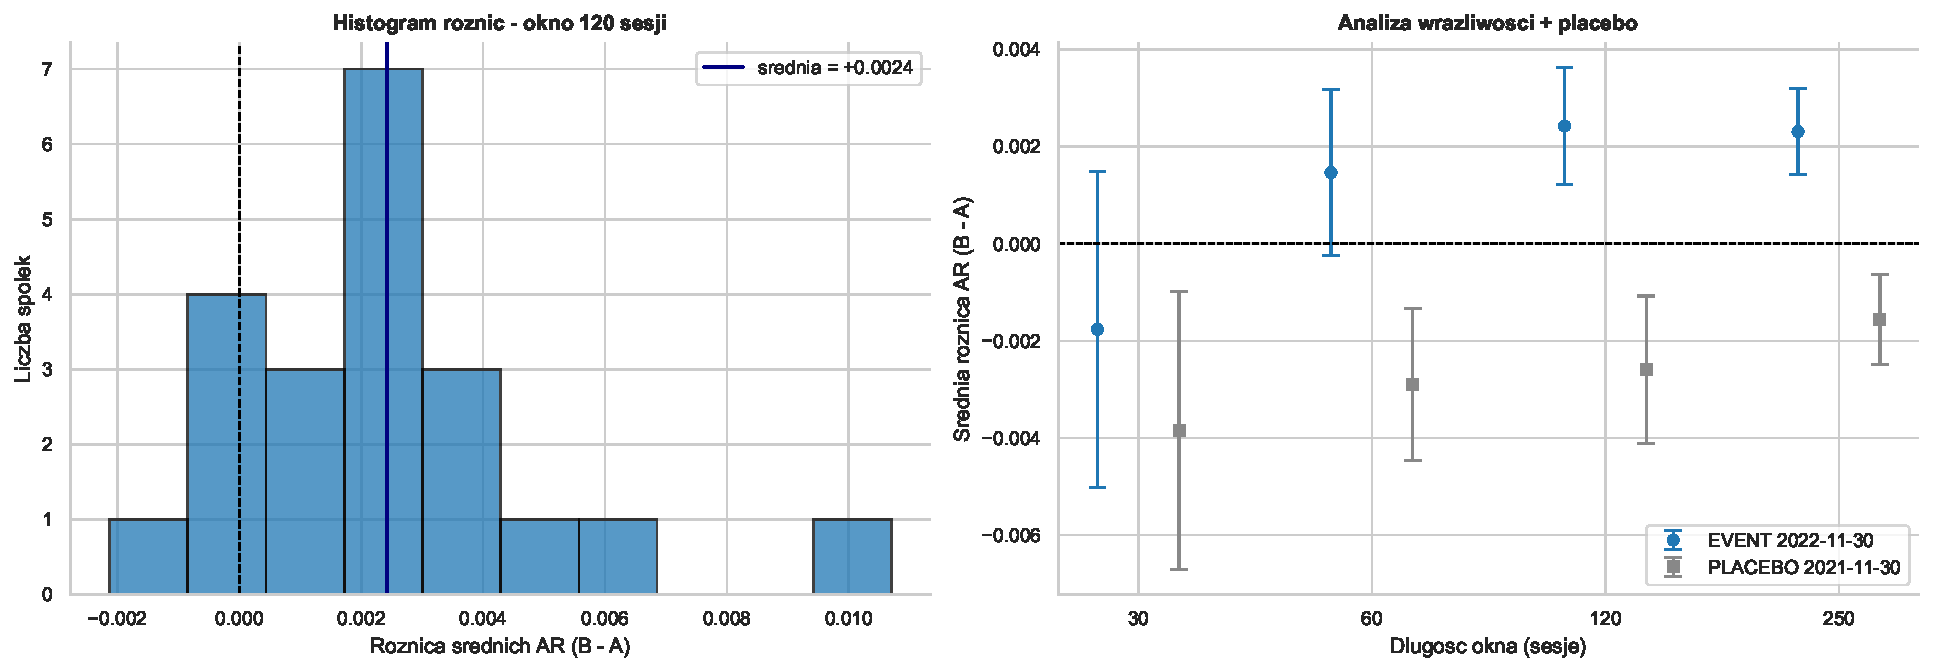
\includegraphics[width=\textwidth]{../figures/task3_sensitivity_placebo.pdf}
\end{center}

\paragraph{Event-window CAR --- portfele EW per grupa wokół 30.11.2022.}
\begin{center}
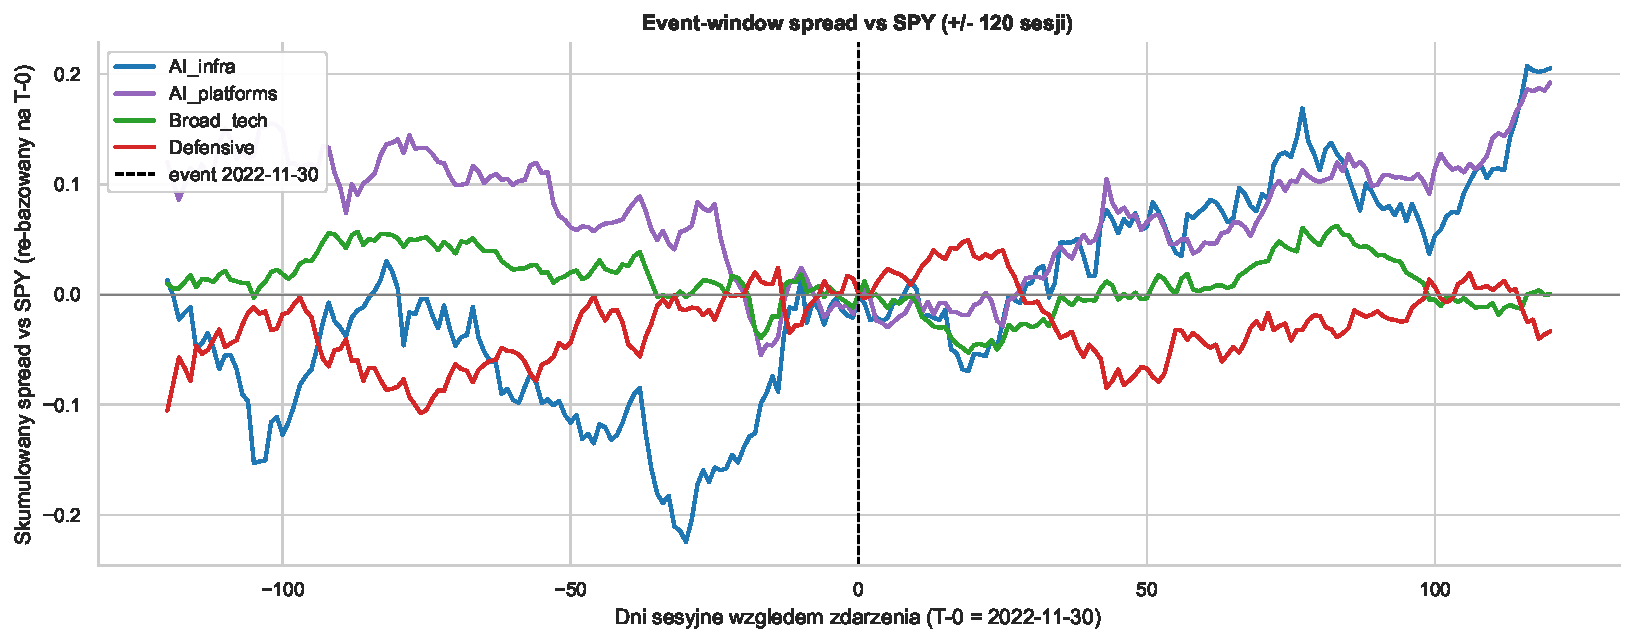
\includegraphics[width=\textwidth]{../figures/extra_event_window_CAR.pdf}
\end{center}

\subsection{Interpretacja}
\begin{itemize}
  \item \textbf{Zmienna}: $d_i = \bar{AR}_i^{(B)} - \bar{AR}_i^{(A)}$ dla
        $n = 21$ spółek z grupy AI; $\bar{AR}$ to średni dzienny abnormal return
        (vs SPY) w oknie $K$ sesji.
  \item \textbf{Test zastosowany}: Wilcoxon signed-rank (główny, bo Shapiro
        odrzucił normalność dla okna 120) + paired $t$-test (wspierający).
  \item \textbf{Wynik (okno bazowe $K = 120$)}: $\bar d = +0{,}243$ p.p.
        \emph{dziennie}; 95\% CI $[+0{,}123;\ +0{,}363]$ p.p.; $d_z = +0{,}92$
        (duży efekt); Wilcoxon $p = 8{,}4 \cdot 10^{-5}$.
  \item \textbf{Decyzja statystyczna}: odrzucamy $H_0$ z wysokim marginesem dla
        okien 120 i 250 sesji. Dla okna 60 efekt graniczny ($p = 0{,}076$),
        dla okna 30 nieistotny. Jest to spójne z interpretacją, że rynek nie
        wycenił całej premii AI natychmiast, lecz w kolejnych miesiącach po
        zdarzeniu.
  \item \textbf{Placebo}: dla 30.11.2021 efekt jest \emph{ujemny i istotny}
        we wszystkich oknach. Kierunek przeciwny do eventu rzeczywistego
        wzmacnia interpretację czasowego związku z 30.11.2022 i ogranicza
        ryzyko, że dodatni wynik jest prostym artefaktem wybranej metody
        przed--po. Nie jest to jednak samodzielny dowód przyczynowości.
  \item \textbf{Interpretacja ekonomiczna}: po publicznej premierze ChatGPT
        spółki z grupy AI generowały średnio o ok. 0{,}24 p.p. \emph{dziennie}
        wyższy abnormal return niż w analogicznym oknie przed premierą. Prosta
        annualizacja tej średniej ($0{,}243\% \times 252$) daje ok. 61 p.p.
        rocznie, dlatego wynik należy traktować jako bardzo duży efekt
        historyczny, a nie jako prognozę przyszłych stóp zwrotu. Dla okna
        120 sesji liniowa kumulacja odpowiada ok. 29 p.p. przewagi abnormal
        returnu.
\end{itemize}

\paragraph{Ograniczenia.}
Analiza ma charakter \emph{uproszczonego testu A/B przed--po}: nie modeluje
oczekiwanego abnormal returnu względem modelu czynnikowego (Fama-French
3/5 czynników); raportujemy AR jedynie względem SPY. Wybór grupy zdarzeniowej
(infra + platforms) jest definicyjny --- nie jest to próba losowa.

\cautionbox{Test A/B przed--po jest czytelny i intuicyjny, ale nie kontroluje
pełnego zestawu czynników rynkowych. Wynik należy traktować jako mocny sygnał
historyczny, a nie jako dowód przyczynowości ani prognozę przyszłych zwrotów.}

\clearpage
% =====================================================================
\section*{Wnioski końcowe i decyzja inwestora}

\paragraph{Wnioski statystyczne.}
\begin{itemize}
  \item \textbf{Zad 1.} Welch t-test odrzuca $H_0$ ($p = 0{,}0079$,
        Hedges' $g = 0{,}59$): portfel AI infrastructure ma istotnie wyższą
        średnią miesięczną nadwyżkę względem SPY niż portfel Defensive
        po 30.11.2022 (+3{,}7 p.p./miesiąc).
  \item \textbf{Zad 2.} ANOVA odrzuca $H_0$ dla obu zmiennych: Sharpe
        ($F = 4{,}96;\ p = 0{,}005;\ \omega^2 = 0{,}23$) i CAPM $\alpha$
        ($F = 7{,}62;\ p = 4 \cdot 10^{-4};\ \omega^2 = 0{,}33$). Dla Sharpe
        Tukey wskazuje istotną przewagę AI infrastructure nad wszystkimi
        pozostałymi grupami; dla CAPM $\alpha$ przewaga AI infrastructure jest
        istotna względem AI platforms i Broad tech, ale nie względem Defensive.
  \item \textbf{Zad 3.} Wilcoxon ($K = 120$): $p = 8{,}4 \cdot 10^{-5}$;
        $\bar d = +0{,}24$ p.p./dzień; 95\% CI $[+0{,}12;\ +0{,}36]$ p.p.;
        $d_z = +0{,}92$. Placebo test daje efekt w kierunku przeciwnym, co
        wzmacnia interpretację czasowego związku wyniku z datą zdarzenia, ale
        nie stanowi samodzielnego dowodu przyczynowości.
\end{itemize}

\paragraph{Decyzja inwestora --- praktyczny take-away.}
\begin{itemize}
  \item Trzy niezależne testy zgodnie wspierają tezę \emph{AI Boom Premium} ---
        ale przede wszystkim w segmencie infrastruktury (półprzewodniki, sprzęt),
        nie w platformach chmurowych.
  \item Premium wiąże się z istotnie wyższym ryzykiem: portfel AI infrastructure
        miał volatility 50\% rocznie (vs 19\% Defensive) i max drawdown $-58\%$.
        Inwestor awersyjny wobec ryzyka powinien stosować mniejszą wagę
        w portfelu niż sugerowałaby sama wielkość średniej nadwyżki.
  \item Wyniki są \emph{ex post} i odzwierciedlają konkretny okres 2021--2026.
        Standardowe ostrzeżenie: ,,past performance is not indicative of future
        results''. Czy premia utrzyma się po fazie szczytowej AI capex ---
        pozostaje otwartą kwestią.
\end{itemize}

% =====================================================================
\section*{Reproducibility note}

\paragraph{Środowisko.} Analizy wykonano w Pythonie. Dokładne wersje bibliotek
należy utrwalać automatycznie w pliku \texttt{requirements.txt} lub przez
\texttt{pip freeze}, zamiast przepisywać je ręcznie do raportu. Kluczowe pakiety:
\texttt{pandas}, \texttt{numpy}, \texttt{scipy}, \texttt{statsmodels},
\texttt{scikit-posthocs}, \texttt{matplotlib}, \texttt{seaborn},
\texttt{yfinance}, \texttt{pyarrow}.

\paragraph{Dane.} Źródło: Yahoo Finance via \texttt{yfinance}. Pobranie:
2026-05-20. Cache lokalny: \texttt{data\_cache/prices.parquet}
(43 tickery $\times$ 1347 dni sesyjnych). Mapowanie ticker $\rightarrow$ grupa:
\texttt{data\_cache/metadata\_tickers.csv}.

\paragraph{Skrypty (kolejność wykonania).}
\begin{enumerate}
  \item \texttt{src/data\_fetch.py} --- pobranie i zapis do parquet.
  \item \texttt{src/task1\_two\_portfolios.py} --- Zadanie 1.
  \item \texttt{src/task2\_four\_groups.py} --- Zadanie 2 (Sharpe i alpha).
  \item \texttt{src/task3\_paired\_event.py} --- Zadanie 3 (event + placebo).
  \item \texttt{src/plots\_extra.py} --- wykresy zaawansowane.
\end{enumerate}
Moduły wspólne: \texttt{src/common.py} (wczytywanie, log returns, portfele EW,
abnormal returns, RF), \texttt{src/metrics.py} (7 metryk per spółka),
\texttt{src/plot\_utils.py} (style i zapis wykresów).

\paragraph{Ziarno losowe.} Bootstrap w Zad. 1 używa \texttt{numpy.random.default\_rng(seed=42)}
i $B = 10\,000$ powtórzeń. Pozostałe analizy są deterministyczne.

\paragraph{Repozytorium.}
\href{https://github.com/Smalou/metody_badania_w_finansach}{\texttt{github.com/Smalou/metody\_badania\_w\_finansach}}
--- pełny kod, dane cache i źródło LaTeX dostępne publicznie.

% =====================================================================
\section*{Limitations}

\begin{itemize}
  \item \textbf{Selection bias / próby celowe}. Wszystkie cztery grupy spółek
        dobrane są ręcznie na bazie eksperckiej oceny ekspozycji na AI --- nie
        są losowymi próbami z populacji. Wnioski dotyczą tej konkretnej próby.
  \item \textbf{Niejednorodność wewnątrzgrupowa}. Grupy Broad tech i Defensive
        zawierają spółki o zróżnicowanych modelach biznesowych, co zwiększa
        wewnętrzną wariancję metryk.
  \item \textbf{Single-factor benchmark}. Abnormal returns liczone są jako
        prosty spread względem SPY. Nie kontrolujemy ekspozycji na czynniki
        Fama-French (HML, SMB, momentum) ani na czynniki sektorowe.
  \item \textbf{Definicja zdarzenia}. Premiera ChatGPT (30.11.2022) jest
        symbolicznym punktem startu boomu AI, ale realna fala kapitałowa
        następowała stopniowo przez kolejne 6--12 miesięcy. Stąd wrażliwość
        wyników Zad. 3 na długość okna.
  \item \textbf{Częściowy ostatni miesiąc}. W Zad. 1 maj 2026 jest miesiącem
        częściowym. Nie zmienia to głównej logiki testu, ale w wersji produkcyjnej
        warto dodać wariant z wykluczeniem niepełnego miesiąca.
  \item \textbf{Dane \texttt{yfinance}}. Ceny są korygowane wstecznie (split,
        dywidenda); dostawca może okresowo modyfikować historyczne wartości.
        Cache lokalny zapewnia reprodukowalność tej analizy, ale ponowne
        pobranie może dać minimalnie inne wyniki.
  \item \textbf{Spojrzenie ex-post}. Cały kierunek hipotezy (,,AI Premium'')
        jest motywowany obserwacjami z lat 2023--2025. Test jest
        konfirmacyjny, nie predykcyjny.
\end{itemize}

% =====================================================================
\section*{Dodatek --- wykresy uzupełniające}

\paragraph{Heatmapa korelacji dziennych log-zwrotów.}
\begin{center}
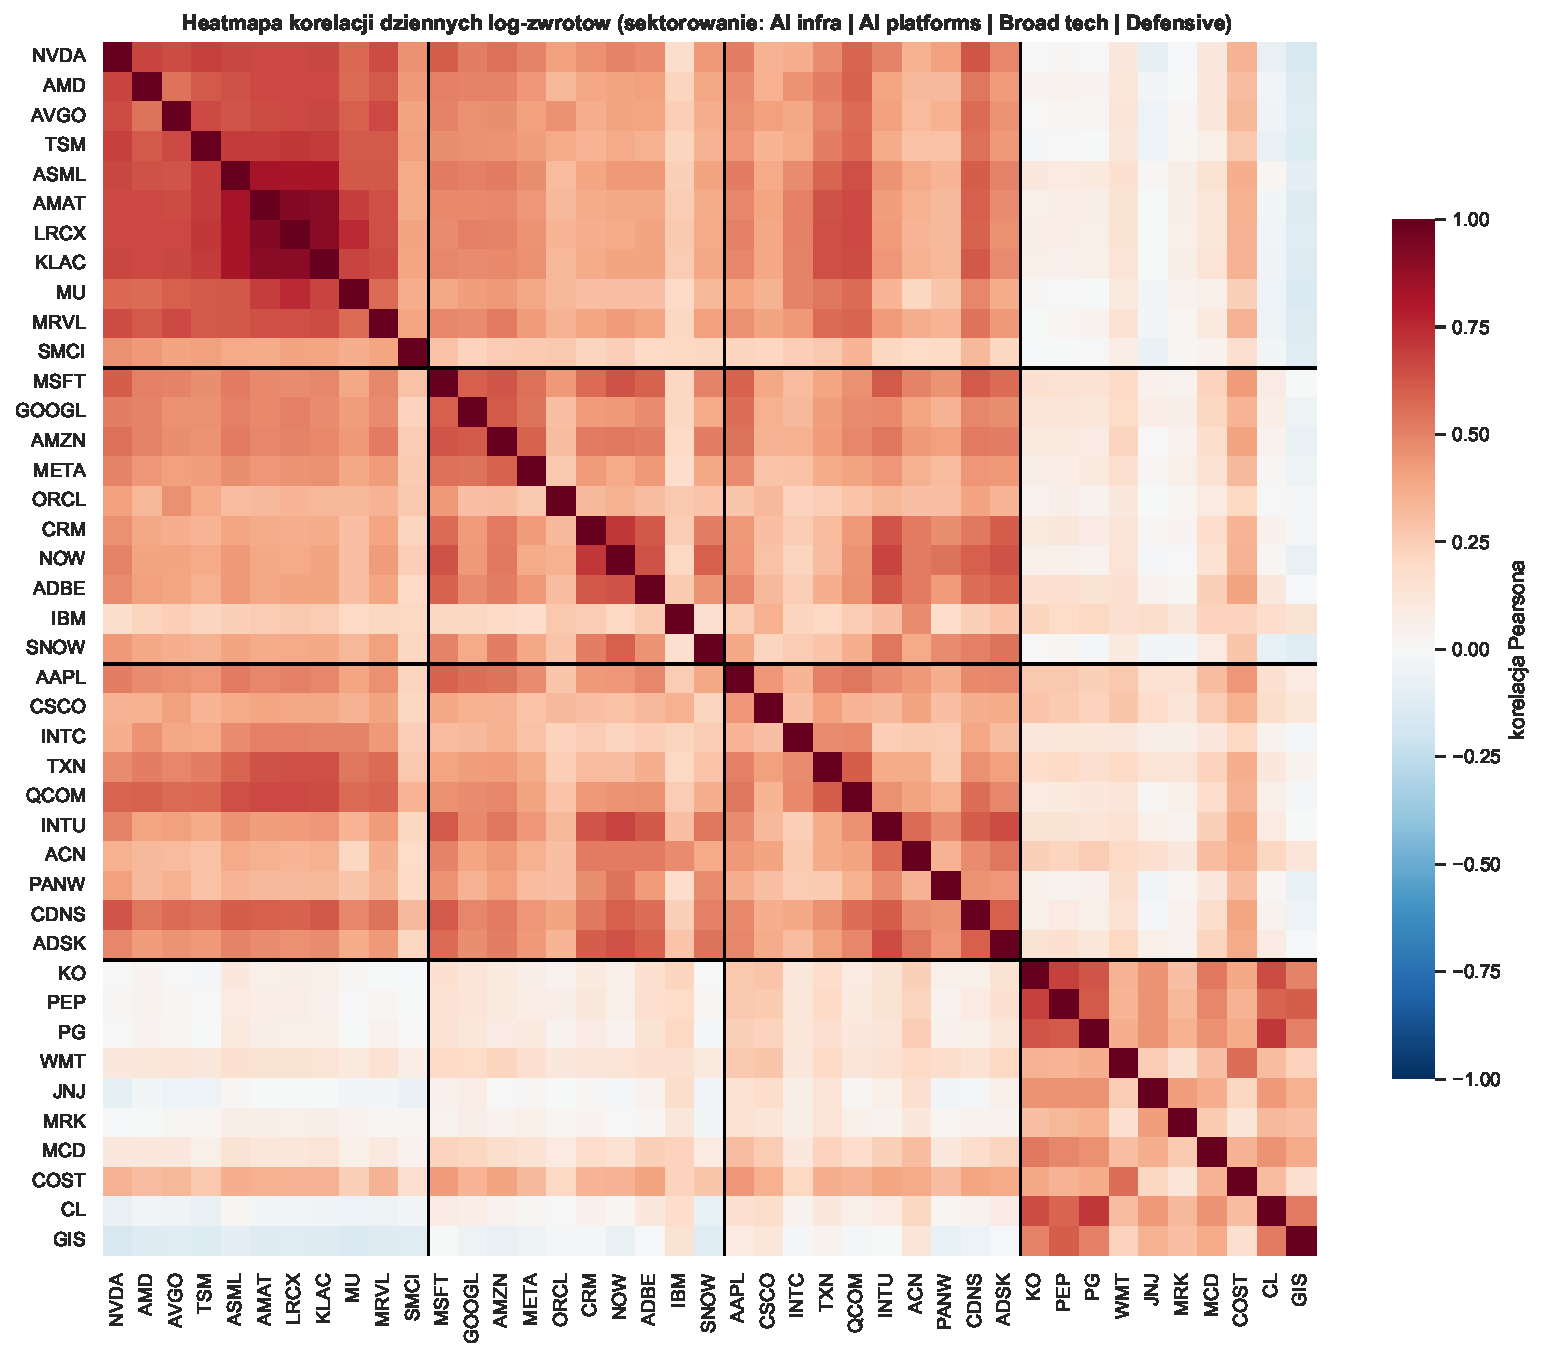
\includegraphics[width=0.95\textwidth]{../figures/extra_corr_heatmap.pdf}
\end{center}
Wizualnie widoczne są bloki wysokiej korelacji wewnątrz grup AI (infra,
platforms) oraz niska korelacja grupy Defensive z technologiami.

\paragraph{Rolling annualized volatility (okno 63 sesji).}
\begin{center}
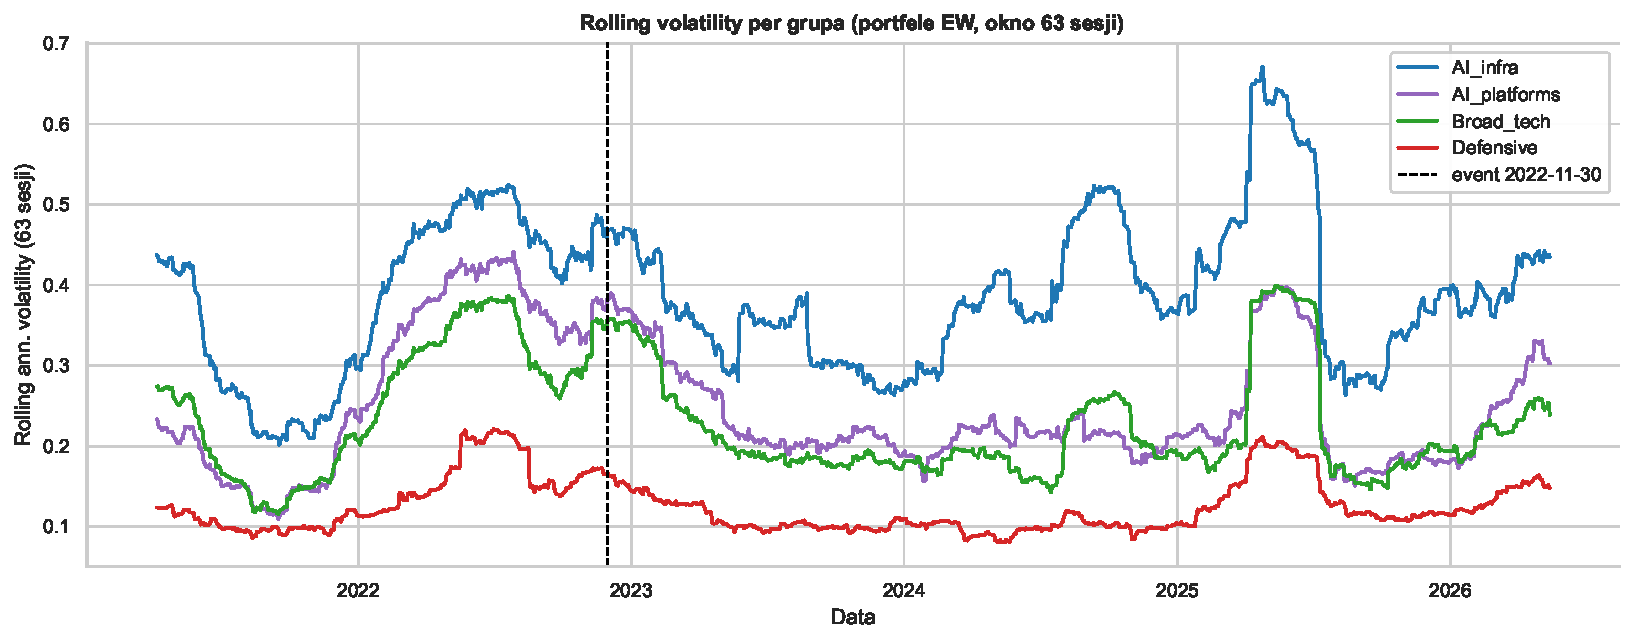
\includegraphics[width=0.95\textwidth]{../figures/extra_rolling_vol.pdf}
\end{center}
AI infrastructure utrzymuje najwyższy poziom zmienności w całym okresie,
ze szczytami wokół wybuchu AI capex 2023 i fazy korekt 2024--2025.

% =====================================================================
\section*{Bibliografia}
\begin{enumerate}
  \item Sharpe, W. F. (1994). The Sharpe Ratio. \emph{The Journal of Portfolio
        Management}, 21(1), 49--58.
  \item Sortino, F. A., \& Price, L. N. (1994). Performance measurement in a
        downside risk framework. \emph{Journal of Investing}, 3(3), 59--64.
  \item Welch, B. L. (1947). The generalization of ``Student's'' problem when
        several different population variances are involved. \emph{Biometrika},
        34(1--2), 28--35.
  \item Games, P. A., \& Howell, J. F. (1976). Pairwise multiple comparison
        procedures with unequal $N$'s and/or variances. \emph{Journal of
        Educational Statistics}, 1(2), 113--125.
  \item Cohen, J. (1988). \emph{Statistical Power Analysis for the Behavioral
        Sciences}, 2nd ed., Lawrence Erlbaum Associates.
  \item Hedges, L. V. (1981). Distribution theory for Glass's estimator of
        effect size and related estimators. \emph{Journal of Educational
        Statistics}, 6(2), 107--128.
  \item MacKinlay, A. C. (1997). Event Studies in Economics and Finance.
        \emph{Journal of Economic Literature}, 35(1), 13--39.
  \item Fama, E. F., \& French, K. R. (1993). Common risk factors in the
        returns on stocks and bonds. \emph{Journal of Financial Economics},
        33(1), 3--56.
  \item OpenAI (2022). \emph{Introducing ChatGPT},
        \url{https://openai.com/index/chatgpt/}.
  \item Yahoo Finance / \texttt{yfinance} --- dokumentacja API,
        \url{https://github.com/ranaroussi/yfinance}.
\end{enumerate}

\end{document}
